% !TEX encoding = UTF-8 Unicode
\documentclass[a4paper,12pt]{article}
\usepackage{polski}
\usepackage[utf8]{inputenc}
\usepackage{graphicx}
\usepackage{float}
\usepackage{rotating}
\usepackage{caption}
\usepackage{subcaption}
\usepackage{pdfpages}
\usepackage{ucs}
\usepackage{amsmath}
\usepackage{amsfonts}
\usepackage{amssymb}
\usepackage{ucs}
\usepackage{epstopdf}
\usepackage{epsfig}
\usepackage{lmodern}
\usepackage{url}

\begin{document}
% Strona tytułowa
\begin{titlepage}
\begin{center}
\vspace*{1cm}
{ \Large Sprawozdanie }\\[1cm]

%{ \Large \textsc{\\ robota mobilnego} }\\[2cm]

{ \large \textbf{Budowa modelu regresji liniowej} }\\
Semestr letni 2017/2018\\[2cm]

\Large
\textbf{Autor:}\\
Artur Błażejewski, 200541\\


\vfill
\Large
Politechnika Wrocławska\\
\large
Wydział Elektroniki\\
Automatyka i Robotyka\\
ARR
\end{center}
\end{titlepage}

\section{Miary skuteczności modelu}
	Do porównywania jakości regresji liniowej wykorzystano błąd MSE (błąd średnio kwadratowy) oraz współczynnik determinacji $R^2$ (najlepsza wartość 1.0). W obliczaniu skuteczności modelu zostanie wykorzystana walidacja krzyżowa z pięcioma iteracjami.

\section{Metoda}
	Zastosowano metodę LinearRegresion z biblioteki sklearn z pakietu linear\_model.

\section{Przygotowanie danych}
	Z danych usunięto wiersze, w których brakowało rekordów lub posiadały one błędną formę.
	
	Przed uczeniem modelu dane są zawsze przetasowane w niezmienny sposób oraz podzielone na dwa zbiory:
	\begin{itemize}
		\item Zbiór treningowy - 80\% całego zbioru danych
		\item Zbiór testowy
	\end{itemize}
	
	W celu oczyszczenia danych z próbek niepozwalających na poprawne przewidywanie wykorzystano wiedzę zawartą w artykule\cite{slave_article} gdzie sugerowano, że cena niewolnika stanowi wielomian szóstego stopnia.
	
	\subsection{Oczyszczanie danych}
		\begin{tabular}{lll}
			Usunięto	&	MSE		&	$R^2$\\
			Nic			&	-5134398	&	-0.08\\
			Cena powyżej 2000\$ \ref{price}	&	-113938	&	0.29\\
			Sprzedaż powyżej jednej osoby \ref{wiecej_niz_jeden}
			&	-96511	&	0.33\\		
			
		\end{tabular}
	
		\subsubsection{Cena}
		\label{price}
		Histogram \ref{hist} pokazuje rozkład ceny bez edycji, po usunięciu rekordów powyżej 10 tys. otrzymujemy \ref{hist10k} a gdy usunięto wartości powyżej 2 tys. \ref{hist2} i dopiero ten rozkład cen przypomina normalny dlatego zdecydowano się na przedział do 2 tys.
		
		\subsubsection{Sprzedaż w zestawach}
		\label{wiecej_niz_jeden}
			Usunięto wszystkie transakcje dotyczące więcej niż jednej osoby, ponieważ wpływają one negatywnie na wynik przewidywania. W pakiecie są sprzedawani niewolnicy w różnym wieku, a cena jest podana jedna dla wszystkich. Uśrednienie ceny nie przyniosłoby pozytywnych rezultatów.
		
		
		\begin{figure}[h]
					\centering
					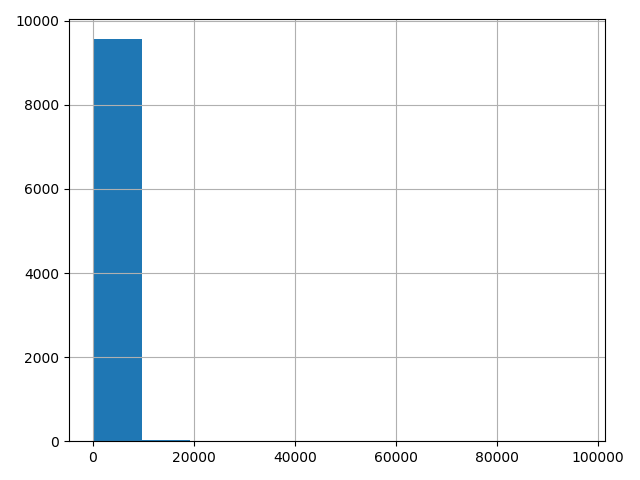
\includegraphics[scale=0.6]{obrazy/hist.png} 
					\caption{histogram cen}
					\label{hist}
		\end{figure}
		\begin{figure}[h]
					\centering
					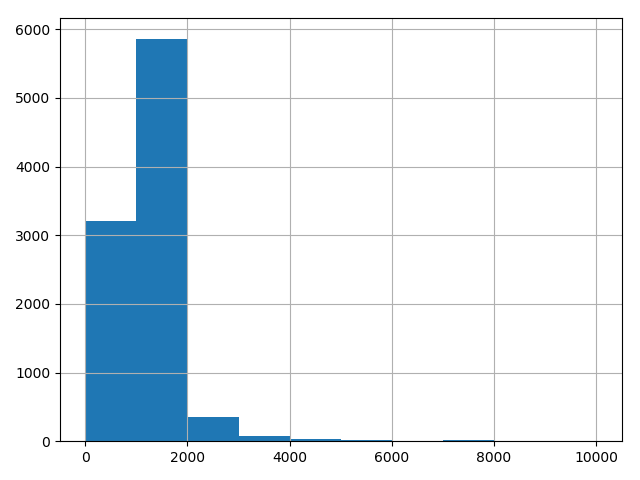
\includegraphics[scale=0.6]{obrazy/hist10.png} 
					\caption{histogram cen w przedziale do 10 tys.}
					\label{hist10k}
		\end{figure}
		\begin{figure}[h]
			\centering
			\includegraphics[scale=0.6]{obrazy/hist2.png} 
			\caption{histogram cen w przedziale do 2 tys.}
			\label{hist10k}
		\end{figure}
		
\section{Analiza błędów}
	Na podstawie krzywej uczenia pokazanej na rysunku \ref{learning_curve} należy stwierdzić, że model posiada wysokie odchylenie, co może oznaczać, że cierpi na niedouczenie i pożądane jest wprowadzenie nowych cech.
	
		\begin{figure}[h]
					\centering
					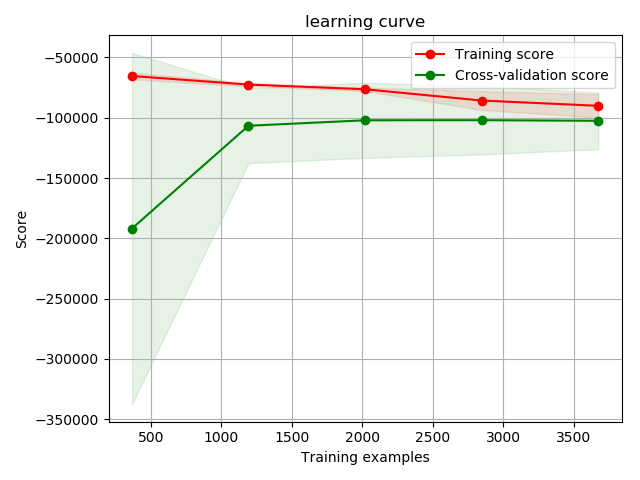
\includegraphics[scale=0.6]{obrazy/learning_curve.png} 
					\caption{Wykres błędu MSE dla zbioru treningowego i walidacyjnego w zależności od wielkości zbioru treningowego}
					\label{learning_curve}
		\end{figure}	
		
\section{Poprawa modelu poprzez dodania nowych cech}		
	\subsection{Wyniki przewidywania}
		\begin{tabular}{lll}
			Cecha			&	MSE		&	$R^2$\\
			Płeć \ref{sex}	&	-93751	&	0.35\\
			Płeć/wiek \ref{age_sex}	&	-91862	&	0.37\\
			Data sprzedaży	\ref{sale_data}	&	-82296	&	0.43\\
			Pochodzenie kupującego \ref{buyer_country}	&	-81343	&	0.43\\
			Pochodzenie sprzedającego	\ref{saller_country}	&	-81267	&	0.43\\
			Kolor skóry	\ref{color}	&	-81116	&	0.44\\
			Kolor skóry	modyfikacja \ref{color_female}	&	-81009	&	0.44\\
			
				
		\end{tabular}

	\subsection{Cechy modelu}
		\subsubsection{Wiek}
			Poddano analizie wpływ wartości wielomianu na wielkość błędu i potwierdzono, że wielomian szóstego stopnia jest optymalny, ponieważ kolejne nie przynosiły znacznej poprawy (poniżej 1\%).
			
		\subsubsection{Płeć}
		\label{sex}
			Ponieważ w zbiorze płeć jest oznaczona jako M oraz F wartości te zmieniono na 1 dla mężczyzn, oraz 0 dla kobiet. Tak sformułowaną cechę dodano do modelu.
		
		\subsubsection{Wiek oraz płeć}
		\label{age_sex}
			Ponieważ najwyższa cena mężczyzn i kobiet przypada na różny wiek, została stworzona cecha, która dla kobiet wynosiła 0, a dla mężczyzn stanowiła wiek. Ponieważ wiek jest funkcją wielomianową, rozważono wielomiany stopnia 1,2,3,4,5,6 i ostatecznie wybrano wielomian stopnia 3.
			
		\subsubsection{Data sprzedaży}
		\label{sale_data}
			Ceny niewolników różniły się znacznie w zależności od pory roku, ponieważ w okresie letnim w Nowym Orleanie panowała żółta febra, mało osób decydowało się na zakup w tym czasie. Ponieważ okres ten obfitował w różne wydarzenia historyczne mające wpływ na cenę, również rok niesie pewne pozytywne informacje w procesie przewidywania.
		
			Ponieważ przewidywanie odbywa się w okresie od października 1956 do sierpnia 1861 cecha jest opisana za pomocą numeru miesiąca zakupu obliczanego wg formuły \ref{obl_data}
			\begin{equation}
			cecha = miesiac + 12*(rok-1956)
				\label{obl_data}
			\end{equation}
		
		\subsubsection{Pochodzenie kupującego}
		\label{buyer_country}
			Cecha ma wartość 1, gdy kupujący jest z Nowego Orleanu, w przeciwnym wypadku 0.
		
		\subsubsection{Pochodzenie sprzedającego}
		\label{saller_country}
			Cecha ma wartość 1, gdy sprzedający jest z Nowego Orleanu, w przeciwnym wypadku 0.
		
		\subsubsection{Kolor skóry}
		\label{color}
			Kolejną cechę stanowi kolor skóry, został zapisany wg wzoru:
			\begin{itemize}
				\item negro = 2
				\item mulatto = 3
				\item griff oraz light griff = 4
				\item yellow = 5
				\item pozostałe kolory oraz brak koloru 1
			\end{itemize}
		
		\subsubsection{Kolor skóry tylko kobiety}
		\label{color_female}
			Wg autorów artykułu\cite{slave_article} kolor skóry ma znacznie większy wpływ na cenę sprzedawanych kobiet. Zmodyfikowano wcześniejszą cechę kolor, ustawiając wartość 0 dla mężczyzn.

\section{Podsumowanie}
	\subsection{Wybór cech}
	\begin{figure}[h]
		\centering
		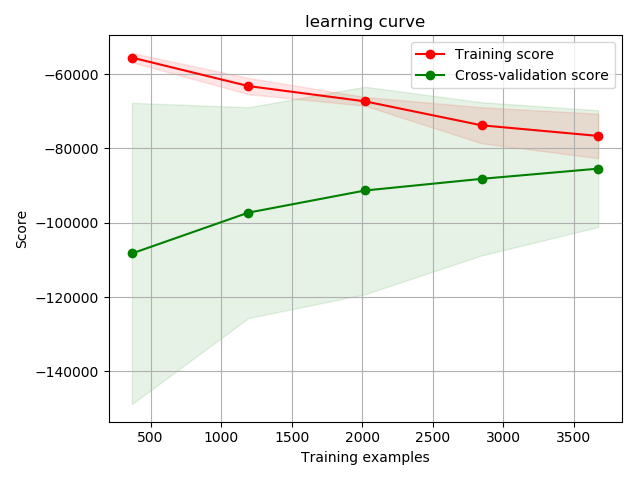
\includegraphics[scale=0.6]{obrazy/learning_curve_new.png} 
		\caption{Wykres błędu MSE dla zbioru treningowego i walidacyjnego w zależności od wielkości zbioru treningowego dla nowo wybranych cech}
		\label{learning_curve_new}
	\end{figure}	
	Na podstawie krzywej uczenia przedstawionej na rysunku \ref{learning_curve_new} wyznaczonej dla modelu wyszkolonego dla wszystkich nowo wybranych cech można stwierdzić, że dostarczenie większej ilości danych powinno spowodować poprawę modelu.
	
	Najlepszy wynik to MSE = 81009, $R^2$ = 0.44 oraz 73 średni błąd 73 (MSE przez wielkość zbioru walidacyjnego).
	
	\subsection{Wyniki dla zbioru testowego}
		Na wcześniej wydzielonym zbiorze testowym otrzymano błąd MSE=115761, $R^2$=0.29 oraz 84 (MSE przez wielkość zbioru walidacyjnego). Na wykresie \ref{test_predict} można zobaczyć rozkład prawdziwych i przewidywanych wartości cen.
		\begin{figure}[h]
			\centering
			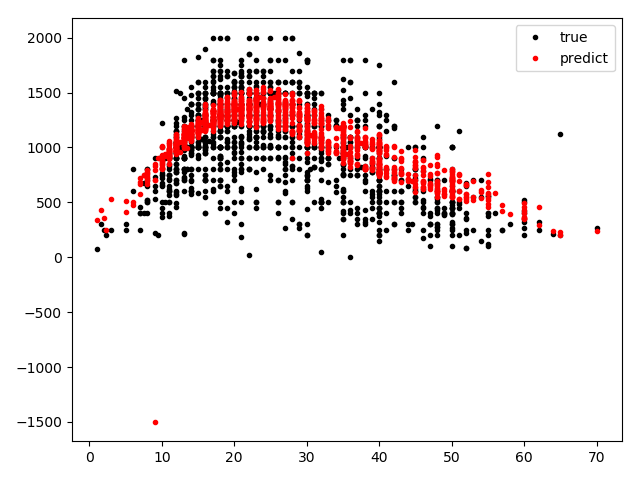
\includegraphics[scale=0.6]{obrazy/test_predict.png} 
			\caption{Przewidywane i prawdziwe wartości ceny w zależności od wieku dla zbioru testowego}
			\label{test_predict}
		\end{figure}	
		Przewidywanie ceny niewolnika wymaga wielu parametrów i jest obarczone dużym błędem, należy się spodziewać, że znaczny wpływ na cenę miały niepodane dane jak wzrost, waga. Otrzymana wartość MSE względem ilości prób testowych pokazuje wzrost błędu dla przypadku testowego względem walidacyjnego. Oznacza to, że model ma pewne problemy z generalizowaniem zagadnienia pomimo wykorzystania zbioru walidacyjnego.
		
\section{Uruchomienie}
	\subsection{Pliki}
	\textbf{Ponieważ nie jest możliwe dodanie plików zadania załączam link z którego można je pobrać \url{https://github.com/artur1993/SlavePrice}}\\
		Do raportu zostały dostarczone następujące pliki:
		\begin{itemize}
			\item LoadDataSet - zawiera funkcje do pobrania danych oczyszczenia z błędów, dodaje i modyfikuje cechy na potrzeby uczenia modelu
			\item LearnModel - pozwala na uzyskanie wartości błędów oraz wyrysowanie krzywej uczenia, plik stworzony na potrzeby dobrania najlepszych parametrów oraz cech modelu
			\item ModelTest - w pliku znajduje się skrypt odpowiedzialny za wyuczenie modelu a następnie przetestowanie go na wydzielonym zestawie testowym
		\end{itemize}
	W plikach LearnModel oraz ModelTest znajduje się zmienna path które zawiera ścieżkę do pliku z danymi (CalomirisPritchett\_data.xlsx) plik pobrany z strony dotyczącej artykułu\cite{slave_article}
	
	Skrypty zostały napisane w języku Python w wersji 3.6.
		
	
\begin{thebibliography}{99}
	\bibitem{slave_article}
	\textit {Betting on Secession: Quantifying Political Events Surrounding Slavery and the Civil War, Charles W. Calomiris and Jonathan Pritchett, \url{https://www.aeaweb.org/articles?id=10.1257/aer.20131483}}

\end{thebibliography}	
		



\end{document}
